\documentclass[10pt, aspectratio=169, handout]{beamer}
\usefonttheme{professionalfonts}

\mode<presentation>
{
  \usetheme{Berkeley}
  \usecolortheme{beaver}
  \usefonttheme{default}
  \setbeamertemplate{navigation symbols}{}
  \setbeamertemplate{caption}[numbered]
} 

\setbeamertemplate{footline}{%
  \leavevmode%
  \hbox{%
    \begin{beamercolorbox}[wd=.85\paperwidth,ht=2.5ex,dp=1ex,left]{author in head/foot}%
      \usebeamerfont{author in head/foot}Digital Signal Processing, Fall 2025%
    \end{beamercolorbox}%
    \begin{beamercolorbox}[wd=.15\paperwidth,ht=2.5ex,dp=1ex,right]{date in head/foot}%
      \hspace*{0.5em}\insertframenumber{} / \inserttotalframenumber\hspace*{0.5em}%
    \end{beamercolorbox}%
  }%
  \vskip0pt%
}

\usepackage[english]{babel}
\usepackage[utf8x]{inputenc}
\usepackage{tikz}
\usepackage{pgfplots}
\usepackage{array}
\usepackage{makecell}
\usepackage{verbatim}
\usepackage{graphicx}
\usepackage{subcaption}
\usepackage{amsfonts}
\usepackage{amsmath}
\usepackage{bm}
\usepackage{epstopdf}
\captionsetup{compatibility=false}

\usetikzlibrary{calc}
\usetikzlibrary{pgfplots.fillbetween, backgrounds}
\usetikzlibrary{positioning}
\usetikzlibrary{pgfplots.groupplots}
\usetikzlibrary{plotmarks}
\usetikzlibrary{calc}
\usetikzlibrary{patterns}
\usetikzlibrary{decorations.pathreplacing}

\usepgfplotslibrary{groupplots}
\pgfplotsset{compat=newest} 

\usepackage{ifthen}
\newboolean{showresults}
\setboolean{showresults}{false}

\usepackage{hyperref}
\hypersetup{
    colorlinks=true,
    linkcolor=blue,
    filecolor=magenta,      
    urlcolor=cyan,
}

\title[ECEN 463/863]{The Inverse z-Transform}
\author{Maxx Seminario}
\institute{University of Nebraska-Lincoln}
\date{October 15, 2025}

\begin{document}
\begin{frame}
  \titlepage
\end{frame}

\section{Introduction}

\begin{frame}{Overview: The Inverse z-Transform}
\begin{itemize}
    \item \textbf{Motivation}: 
    \begin{itemize}
        \item Need to move between time-domain and z-domain representations
        \item Analysis often involves finding z-transform, manipulating, then inverting
        \item Essential for discrete-time signal and system analysis
    \end{itemize}
    
    \item \textbf{Formal Definition}:
    \[
        x[n] = \frac{1}{2\pi j} \oint_C X(z)z^{n-1}dz
    \]
    where $C$ is a closed contour within the ROC
    
    \item \textbf{Practical Methods}:
    \begin{itemize}
        \item Inspection method
        \item Partial fraction expansion
        \item Power series expansion
    \end{itemize}
\end{itemize}
\end{frame}

\section{Inspection Method}

\begin{frame}{Inspection Method}
\textbf{Concept}: Recognize common transform pairs "by inspection"

\vspace{0.3cm}
\textbf{Some Transform Pairs}:
\begin{itemize}
    \item $a^n u[n] \overset{\mathcal{Z}}{\longleftrightarrow} \frac{1}{1 - az^{-1}}, \quad |z| > |a|$
    \item $-a^n u[-n-1] \overset{\mathcal{Z}}{\longleftrightarrow} \frac{1}{1 - az^{-1}}, \quad |z| < |a|$
\end{itemize}

\vspace{0.3cm}
\textbf{Example}: $X(z) = \frac{1}{1 - \frac{1}{2}z^{-1}}$
\begin{itemize}
    \item If $|z| > \frac{1}{2}$: $x[n] = \left(\frac{1}{2}\right)^n u[n]$
    \item If $|z| < \frac{1}{2}$: $x[n] = -\left(\frac{1}{2}\right)^n u[-n-1]$
\end{itemize}

\vspace{0.3cm}
\textbf{Key Point}: ROC determines which sequence! Same $X(z)$ can represent different sequences.
\end{frame}

\section{Partial Fraction Expansion}

\begin{frame}{Partial Fraction Expansion: Overview}
\textbf{For Rational z-Transforms}:
\[
    X(z) = \frac{\sum_{k=0}^{M} b_k z^{-k}}{\sum_{k=0}^{N} a_k z^{-k}} = \frac{b_0}{a_0} \frac{\prod_{k=1}^{M}(1 - c_k z^{-1})}{\prod_{k=1}^{N}(1 - d_k z^{-1})}
\]

\vspace{0.3cm}
\textbf{General Procedure}:
\begin{enumerate}
    \item Factor denominator to find poles $d_k$
    \item Determine expansion form:
    \begin{itemize}
        \item $M < N$: $X(z) = \sum_{k=1}^{N} \frac{A_k}{1 - d_k z^{-1}}$
        \item $M \geq N$: $X(z) = \sum_{r=0}^{M-N} B_r z^{-r} + \sum_{k=1}^{N} \frac{A_k}{1 - d_k z^{-1}}$
    \end{itemize}
    \item Calculate coefficients: $A_k = (1 - d_k z^{-1})X(z)\Big|_{z=d_k}$
    \item Use ROC to determine sequence type:
    \begin{itemize}
        \item Poles inside inner ROC boundary $\rightarrow$ right-sided
        \item Poles outside outer ROC boundary $\rightarrow$ left-sided
    \end{itemize}
\end{enumerate}
\end{frame}

\begin{frame}{Partial Fractions: Simple Poles Example}
\begin{columns}
\begin{column}{0.5\textwidth}
\textbf{Example}: $X(z) = \frac{1}{(1-\frac{1}{4}z^{-1})(1-\frac{1}{2}z^{-1})}, \quad |z| > \frac{1}{2}$

\vspace{0.3cm}
\textbf{Partial fraction expansion}:
\[
X(z) = \frac{-1}{1-\frac{1}{4}z^{-1}} + \frac{2}{1-\frac{1}{2}z^{-1}}
\]

\vspace{0.3cm}
\textbf{Since ROC is $|z| > \frac{1}{2}$}: Both poles inside ROC $\rightarrow$ right-sided sequences

\vspace{0.3cm}
\textbf{Result}:
\[
x[n] = -\left(\frac{1}{4}\right)^n u[n] + 2\left(\frac{1}{2}\right)^n u[n]
\]
\end{column}
\begin{column}{0.5\textwidth}
\begin{center}
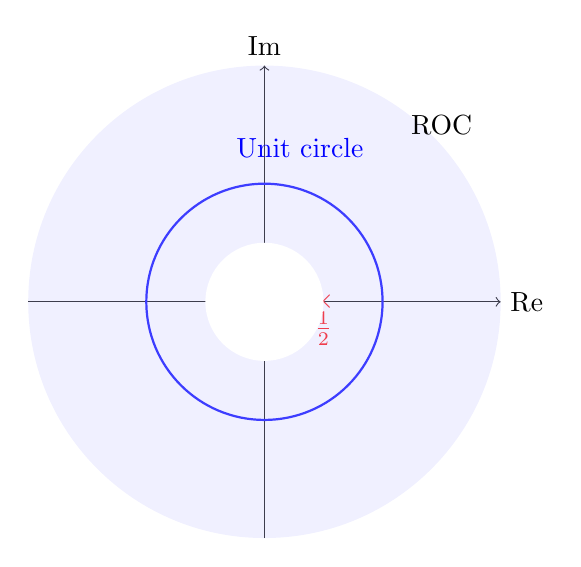
\begin{tikzpicture}[scale=1.5]
    \draw[->] (-2,0) -- (2,0) node[right] {Re};
    \draw[->] (0,-2) -- (0,2) node[above] {Im};
    \draw[thick,blue] (0,0) circle (1);
    \draw[red,thick] (0.25,0) node {$\times$} node[below] {$\frac{1}{4}$};
    \draw[red,thick] (0.5,0) node {$\times$} node[below] {$\frac{1}{2}$};
    \fill[blue!20,opacity=0.3] (0,0) circle (2);
    \fill[white] (0,0) circle (0.5);
    \node at (1.5,1.5) {ROC};
    \node at (0.3,1.3) [blue] {Unit circle};
\end{tikzpicture}
\end{center}
\end{column}
\end{columns}
\end{frame}

\begin{frame}{Partial Fractions: Case $M \geq N$}
\textbf{Example}: $X(z) = \frac{1+2z^{-1}+z^{-2}}{1 - \frac{3}{2}z^{-1} + \frac{1}{2}z^{-2}} = \frac{(1+z^{-1})^2}{(1-\frac{1}{2}z^{-1})(1-z^{-1})}, \quad |z| > 1$

\vspace{0.3cm}
\textbf{Long division yields}: $B_0 = 2$, remainder = $5z^{-1} - 1$

\vspace{0.3cm}
\textbf{Expansion}:
\[
    X(z) = 2 + \frac{-9}{1-\frac{1}{2}z^{-1}} + \frac{8}{1-z^{-1}}
\]

\vspace{0.3cm}
\textbf{Since ROC is $|z| > 1$}: All sequences are right-sided

\vspace{0.3cm}
\textbf{Result}:
\[
    x[n] = 2\delta[n] - 9\left(\frac{1}{2}\right)^n u[n] + 8u[n]
\]
\end{frame}

% \begin{frame}{Partial Fractions: Multiple-Order Poles}
% \textbf{For pole of order $s$ at $z = d_i$}:
% \[
%     \text{Expansion includes: } \frac{C_1}{1-d_i z^{-1}} + \frac{C_2}{(1-d_i z^{-1})^2} + \cdots + \frac{C_s}{(1-d_i z^{-1})^s}
% \]

% \vspace{0.3cm}
% \textbf{Example}: $X(z) = \frac{1}{(1-\frac{1}{2}z^{-1})^2(1-\frac{1}{4}z^{-1})}$

% \vspace{0.3cm}
% \textbf{Transform pairs for multiple poles}:
% \begin{itemize}
%     \item $\frac{1}{(1-az^{-1})^2} \overset{\mathcal{Z}}{\longleftrightarrow} (n+1)a^n u[n]$ for $|z| > |a|$
%     \item $\frac{az^{-1}}{(1-az^{-1})^2} \overset{\mathcal{Z}}{\longleftrightarrow} na^n u[n]$ for $|z| > |a|$
% \end{itemize}

% \vspace{0.3cm}
% \textbf{Coefficient formulas}:
% \begin{itemize}
%     \item $C_s = (1-d_i z^{-1})^s X(z)\Big|_{z=d_i}$
%     \item $C_{s-1} = \frac{d}{dz}[(1-d_i z^{-1})^s X(z)]\Big|_{z=d_i}$
%     \item Continue derivatives for lower-order terms
% \end{itemize}
% \end{frame}

\section{Power Series Expansion}

\begin{frame}{Power Series Expansion}
\textbf{Direct from Definition}: $X(z) = \sum_{n=-\infty}^{\infty} x[n]z^{-n}$

\vspace{0.3cm}
\textbf{Example 1}:
\begin{itemize}
    \item $X(z) = z^2(1-\frac{1}{2}z^{-1})(1+z^{-1})(1-z^{-1}) = z^2 - \frac{1}{2}z - 1 + \frac{1}{2}z^{-1}$
    \item $x[n] = \delta[n+2] - \frac{1}{2}\delta[n+1] - \delta[n] + \frac{1}{2}\delta[n-1]$
\end{itemize}

% \vspace{0.3cm}
% \textbf{Example 2 - Transcendental}:
% \begin{itemize}
%     \item $X(z) = \log(1 + az^{-1}) = \sum_{n=1}^{\infty} \frac{(-1)^{n+1}a^n z^{-n}}{n}$ for $|z| > |a|$
%     \item $x[n] = \begin{cases}
%         \frac{(-1)^{n+1}a^n}{n}, & n \geq 1 \\
%         0, & n \leq 0
%     \end{cases}$
% \end{itemize}

% \vspace{0.3cm}
% \textbf{Long Division}:
% \begin{itemize}
%     \item ROC exterior $\rightarrow$ divide for powers of $z^{-1}$ (right-sided)
%     \item ROC interior $\rightarrow$ divide for powers of $z$ (left-sided)
% \end{itemize}
\end{frame}

\begin{frame}{Example: Complete Inverse Transform}
\begin{columns}
\begin{column}{0.5\textwidth}
\textbf{Given}: 
\[X(z) = \frac{1 + z^{-1}}{(1-\frac{1}{2}z^{-1})(1+\frac{1}{4}z^{-1})}\]
ROC: $\frac{1}{4} < |z| < \frac{1}{2}$

% \vspace{0.3cm}
\textbf{Partial fractions}:
\[
    X(z) = \frac{3}{1-\frac{1}{2}z^{-1}} + \frac{-2}{1+\frac{1}{4}z^{-1}}
\]

\vspace{-0.3cm}
\textbf{ROC analysis}:
\begin{itemize}
    \item Pole at $\frac{1}{2}$ outside ROC $\rightarrow$ left-sided
    \item Pole at $-\frac{1}{4}$ inside ROC $\rightarrow$ right-sided
\end{itemize}

% \vspace{0.3cm}
\textbf{Result}:
\[
    x[n] = -3\left(\frac{1}{2}\right)^n u[-n-1] - 2\left(-\frac{1}{4}\right)^n u[n]
\]
\end{column}
\begin{column}{0.5\textwidth}
\begin{center}
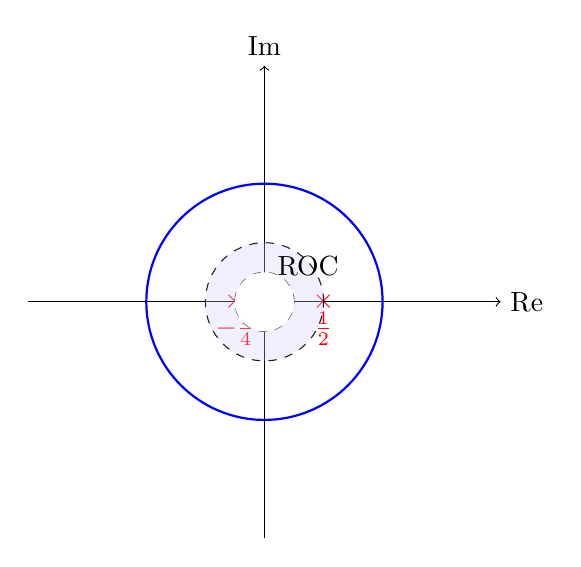
\begin{tikzpicture}[scale=1.5]
    \draw[->] (-2,0) -- (2,0) node[right] {Re};
    \draw[->] (0,-2) -- (0,2) node[above] {Im};
    \draw[thick,blue] (0,0) circle (1);
    \draw[red,thick] (0.5,0) node {$\times$} node[below] {$\frac{1}{2}$};
    \draw[red,thick] (-0.25,0) node {$\times$} node[below] {$-\frac{1}{4}$};
    \draw[dashed] (0,0) circle (0.25);
    \draw[dashed] (0,0) circle (0.5);
    \fill[blue!20,opacity=0.3] (0,0) circle (0.5);
    \fill[white] (0,0) circle (0.25);
    \node at (0.37,0.3) {ROC};
\end{tikzpicture}
\end{center}
\end{column}
\end{columns}
\end{frame}

\section{Summary}

\begin{frame}{Summary of Inverse z-Transform Methods}
\textbf{1. Inspection Method}:
\begin{itemize}
    \item Best for simple, recognizable forms
    % \item Requires familiarity with transform pairs
    % \item Quick but limited applicability
\end{itemize}

\vspace{0.3cm}
\textbf{2. Partial Fraction Expansion}:
\begin{itemize}
    \item Most useful for rational functions
    \item Systematic procedure for simple and multiple poles
    \item ROC critical for determining sequence type
\end{itemize}

\vspace{0.3cm}
\textbf{3. Power Series Expansion}:
\begin{itemize}
    \item Direct from definition
    % \item Long division for rational functions
    % \item Can handle transcendental functions
\end{itemize}

\vspace{0.3cm}
\textbf{Key Principle}: ROC determines sequence type
\begin{itemize}
    \item Poles inside inner boundary $\rightarrow$ right-sided sequences
    \item Poles outside outer boundary $\rightarrow$ left-sided sequences
\end{itemize}
\end{frame}

\end{document}